\chapter{Level 1 : Mon premier jeu en Godot}

Pour ce premier contact avec Godot, nous allons tenter de réaliser un petit jeu sans prétention. Il s'agira d'un jeu où il faut attraper certains objets qui tombent du haut de l'écran, tout en évitant certains autres.

\section{Création du projet}

Quand vous lancez Godot, vous serez saluées par un écran comme celui de la figure \ref{lvl1-screen1}. Au premier lancement, il sera vide, mais vous verrez que bientôt il se remplira de tous les projets que vous aurez créés.

\begin{figure}
  \begin{center}
    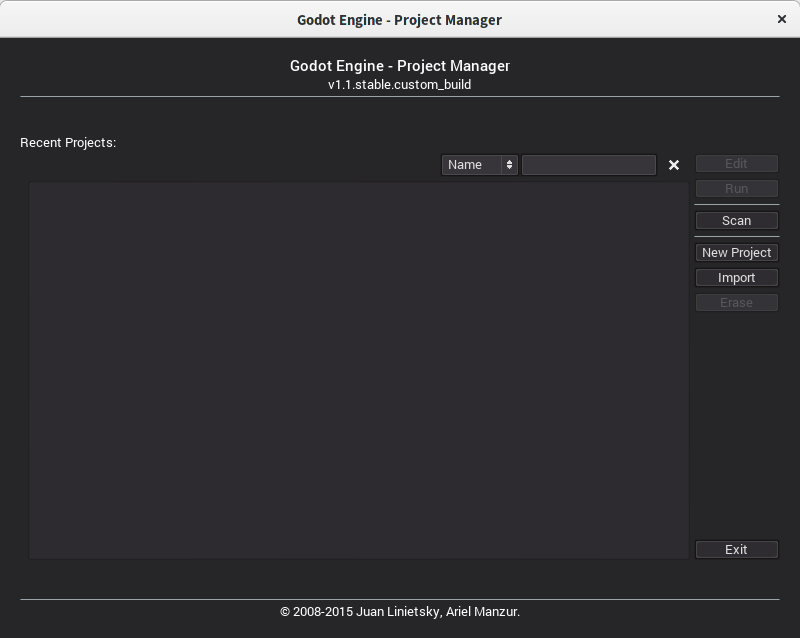
\includegraphics[width=12cm]{img/lvl1-screen1.png}
  \end{center}
  \caption{\label{lvl1-screen1} L'écran de sélection de projets de Godot, sa façon de vous dire bonjour.}
\end{figure}

Le bouton qui nous intéresse plus particulièrement est le bouton \emph{New Project}, qui va nous permettre de... créer un nouveau projet (qui l'eut crû). Vous verrez une popup s'ouvrir, comme sur la figure \ref{lvl1-screen2}.

\begin{figure}
  \begin{center}
    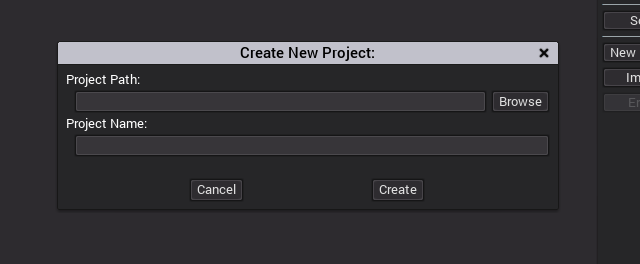
\includegraphics[width=10cm]{img/lvl1-screen2.png}
  \end{center}
  \caption{\label{lvl1-screen2} Un nouveau projet ! Sentez-vous l'excitation qui monte, la hype qui se profile ? Non ? Ah bon...}
\end{figure}

En utilisant le bouton \emph{Browse}, vous pourrez naviguer jusqu'à trouver un endroit parfait pour votre projet. Tous les fichiers du projet seront stockés dans ce dossier. En plus, Godot vous encourage à donner un nom intelligent à votre dossier: par défaut, le nom du dossier sera également le nom du projet. Dans un énorme élan de créativité, j'ai décidé d'appeler mon dossier \codeintext{FallingThings}, d'après le principe de notre jeu.

Une fois la boite de dialogue remplie et validée, vous aurez l'insigne honneur de voir votre nouveau projet apparaître dans la fenêtre de sélection de projets (voir figure \ref{lvl1-screen3}).

\begin{figure}
  \begin{center}
    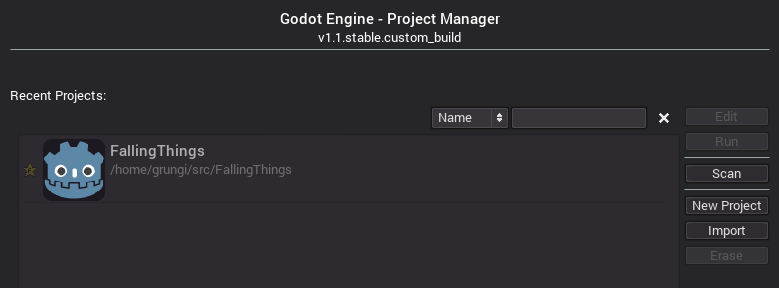
\includegraphics[width=12cm]{img/lvl1-screen3.png}
  \end{center}
  \caption{\label{lvl1-screen3} Et voilà, le projet est maintenant prêt à être ouvert, et le travail va pouvoir commencer.}
\end{figure}

Les choses sérieuses peuvent commencer !

\section{Le Nouveau Monde}

Tels des exploratrices devant les côtes d'une île inconnue, vous avez ouvert votre projet, et vous vous êtes retrouvées devant un écran relativement intimidant. Pas très loin de celui de la figure \ref{lvl1-screen4}.

\begin{figure}
  \begin{center}
    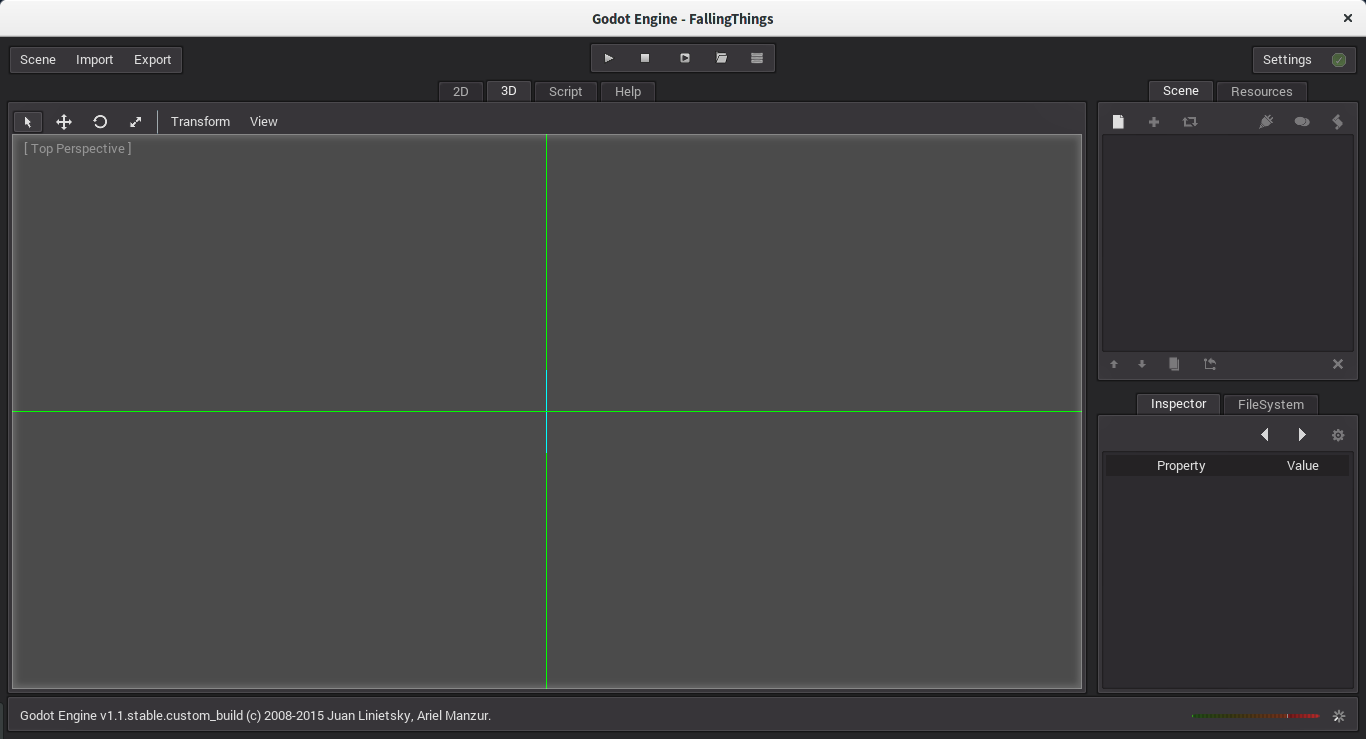
\includegraphics[width=12cm]{img/lvl1-screen4.png}
  \end{center}
  \caption{\label{lvl1-screen4} Des icones, des boutons, des onglets... Bienvenue dans Godot !}
\end{figure}

Pas de panique cependant, c'est plus simple qu'il n'y parait. L'écran est divisé 5 zones principales.

\begin{description}
\item[En haut] : On retrouve des menus, que nous explorerons petit à petit, une barre de boutons qui permettent de lancer le jeu, le stopper, lancer une \emph{scène}, et un bouton sur la droite permettant de modifier certains paramètres de l'éditeur de Godot.
\item[Au centre] : La majeure partie de l'écran est occupée par la zone de travail principal de Godot. Comme un navigateur, elle se présente sous la forme de plusieurs onglets. Le premier de ceux-ci offre une vue 2D de l'application (nous allons souvent l'utiliser), le deuxième sert dans le cadre de projets 3D, le troisième sert à éditer les scripts (le code), et le dernier vous offre l'aide de Godot, bien utile à avoir sous la main.
\item[A droite, en haut] : Vous trouverez là la hiérarchie des \emph{noeuds} présents dans la \emph{scène} en cours. Ce charabia deviendra plus intelligible quand nous parlerons de comment Godot organise les éléments des projets un peu plus loin. Mais retenez que c'est là que vous trouverez les différents éléments qui sont actuellement dans votre jeu. Le second onglet, \emph{Resources}, vous montrera les différentes sources de données (textures, sprites, fichiers sons, ...) qui seront utilisées dans le projet. Nous y reviendrons également plus tard.
\item[A droite, en bas] : Là où l'onglet \emph{Scene} ci-dessus vous montrait la liste des éléments de la \emph{scène}, l'onglet \emph{Inspector} vous renseigne les propriétés de l'objet actuellement sélectionné. Vous pourrez l'utiliser pour définir un grand nombre d'options pour chaque objet. A ses côtés, l'onglet \emph{FileSystem} vous montre simplement un navigateur qui vous permet de parcourir l'arborescence des dossiers de votre projet.
\item[En bas] : Tout en bas de la fenêtre, vous trouverez une barre de statut, qui vous montrera les sorties générées par les commandes que vous utiliserez ou par votre jeu. En cliquant dessus, vous pourrez faire apparaître une zone plus conséquente où vous pourrez voir plus de texte.
\end{description}

Voilà, maintenant que vous êtes familiarisées avec l'organisation générale de l'interface du moteur, il est temps de voir comment utiliser tout cela.

\section{Le \emph{noeud} du problème}

Nous allons maintenant aborder une notion vraiment centrale à l'organisation de Godot: les \emph{noeuds}, ou \emph{nodes} en Anglais.

Le concept va être abstrait pendant quelques lignes, mais nous verrons tout de suite comment l'utiliser en pratique.

Le \emph{noeud} est, dans Godot, l'élément de base avec lequel vous allez créer vos jeux. Depuis un sprite pour représenter un personnage à une source de lumière pour l'éclairer, en passant par une zone déterminant la fin d'un niveau, tout dans Godot est un \emph{noeud}. Plus que ça, les \emph{noeuds} sont définis comme ayant les caractéristiques suivantes:

\begin{enumerate}
\item Un \emph{noeud} a un nom.
\item Un \emph{noeud} possède un ensemble de \emph{propriétés} éditables.
\item Un \emph{noeud} peut faire appel à du code pour remplir son rôle.
\item Un \emph{noeud} peut être ajouté à un autre \emph{noeud} en tant qu'enfant.  
\end{enumerate}

Si les trois premières propriétés sont importantes, c'est la quatrième qui mérite que l'on s'y attarde. En effet, le fait de pouvoir organiser les \emph{noeuds} de façon hiérarchique permet de concevoir des constructions complexes, tout en conservant chaque \emph{noeud} isolé et simple.

Par exemple, on pourrait imaginer un \emph{noeud} pour afficher un personnage 2D, qui aurait pour enfant un \emph{noeud} pour gérer son animation, un autre pour jouer les effets sonores qui lui sont propres, etc. Nous aurons l'occasion de faire usage de cette façon de faire rapidement, vous verrez, c'est très utile ! Mais pour le moment, il suffit de retenir que les \emph{noeuds} peuvent être organisés comme sur la figure \ref{lvl1-nodetree}.

\begin{figure}
  \begin{center}
    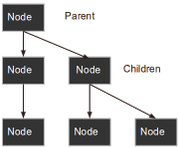
\includegraphics[width=6cm]{img/lvl1-nodetree.png}
  \end{center}
  \caption{\label{lvl1-nodetree} Exemple de hiérarchie de \emph{noeuds}.}
\end{figure}

Mais assez de théorie, passons à l'action !

\section{Première visite au magasin de jouets}

Il est temps de créer nos premiers \emph{noeuds}, et d'enfin voir quelque chose dans notre projet vide. En haut à droite de votre écran, dans l'onglet \emph{Scene}, vous trouverez une petite icône de page blanche, comme sur la figure \ref{lvl1-screen5}. Si vous passez le curseur de votre souris dessus, une info-bulle vous apprendra qu'il s'agit d'un bouton prévu pour créer un nouveau \emph{noeud}, ajoutant en plus un raccourci bien pratique pour faire la même chose : \codeintext{Ctrl + A}.


\begin{figure}
  \begin{center}
    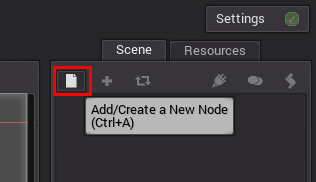
\includegraphics[width=6cm]{img/lvl1-screen5.png}
  \end{center}
  \caption{\label{lvl1-screen5} Le bouton magique.}
\end{figure}

Si vous cliquez sur ledit bouton (ou utilisez le raccourci clavier, selon), une nouvelle fenêtre va s'ouvrir, avec tout un tas de choses dedans. Voyez plutôt à la figure \ref{lvl1-screen6}.

\begin{figure}
  \begin{center}
    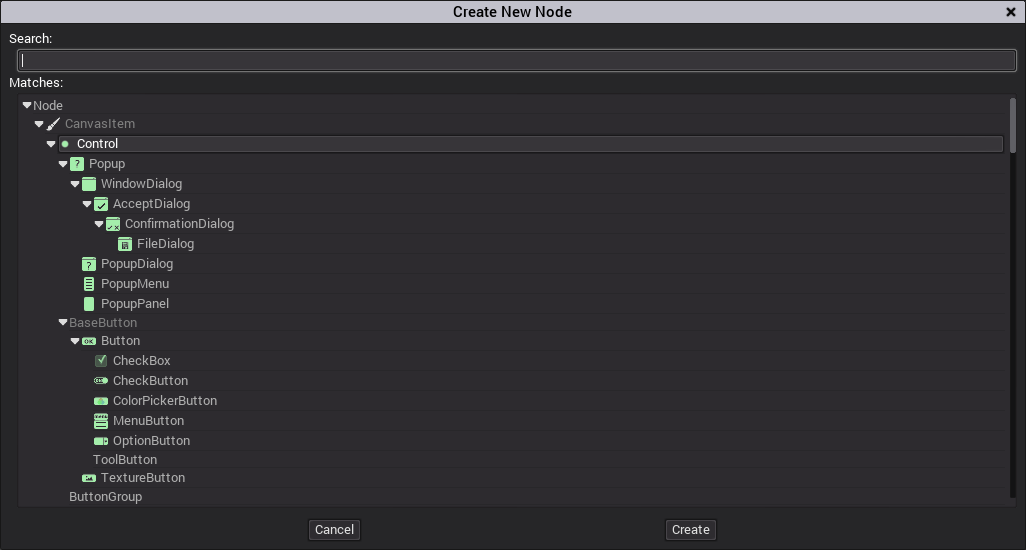
\includegraphics[width=8cm]{img/lvl1-screen6.png}
  \end{center}
  \caption{\label{lvl1-screen6} Votre magasin de jouets perso !}
\end{figure}

Comme dans un vrai magasin, des objets de toutes les couleurs sont en compétition pour votre attention, et sont organisés d'une manière qui, si elle n'est pas apparente de prime abord, l'est à l'usage. La première chose que vous pourrez remarquer est que les différents objets sont principalement regroupés par couleur. Pour vous y retrouver, voici les trois couleurs principales :

\begin{description}
\item[Vert] pour tout ce qui touche aux interfaces utilisateur (boutons, boites de dialogue, ...)
\item[Bleu] pour tout ce qui est 2D. C'est la couleur qui nous sera la plus utile !
\item[Rouge] pour tout ce qui est 3D. Comme expliqué dans le préambule de ce cours, nous n'aurons pas vraiment l'occasion de nous pencher sur le sujet, mais il est bon de savoir ce qui existe dans Godot.
\end{description}

Les autres couleurs sont plus mineures, et moins essentielles (ou ne sont pas dans une catégorie précise).

Spoiler : chaque élément de la liste présentée dans la fenêtre est un type de \emph{noeud} prédéfini dans Godot. Ils obéissent donc tous aux 4 propriétés que nous avons vues plus tôt !

Nous allons donc sans plus tarder partir à la recherche d'un \emph{noeud} qui pourrait nous servir de base pour notre jeu. Il est toujours préférable d'avoir un noeud principal qui contient l'ensemble des éléments d'un niveau (ou ici du jeu entier), et en général il s'agira d'un \emph{noeud} le plus général possible. Ici, le type \codeintext{Node2D} est idéal puisqu'il est le plus simple des \emph{noeuds} 2D. Cherchez-le dans la liste via la barre de recherche au dessus de la fenêtre, ou en parcourant la liste, et appuyez sur \emph{Create}.

\begin{figure}
  \begin{center}
    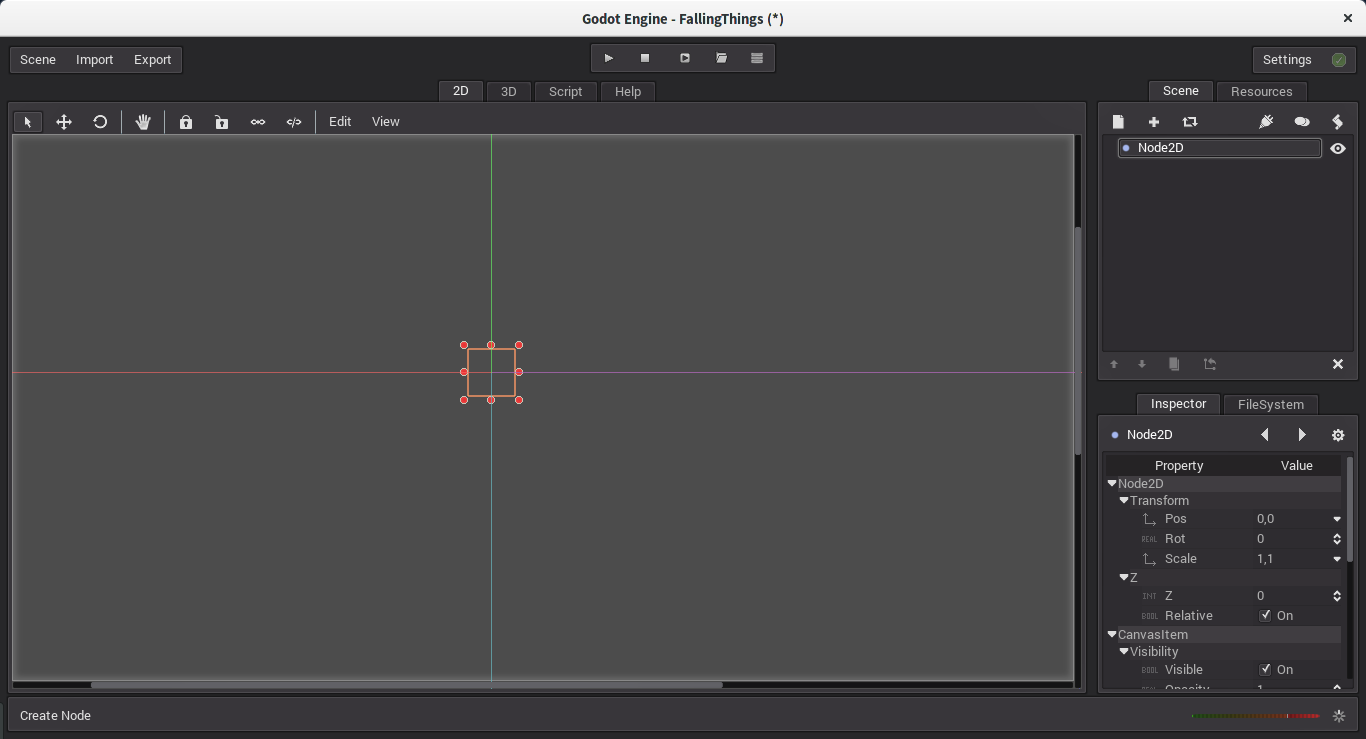
\includegraphics[width=12cm]{img/lvl1-screen7.png}
  \end{center}
  \caption{\label{lvl1-screen7} Notre tout premier noeud ! N'est-il pas joli ?}
\end{figure}

Votre écran devrait ressembler fortement à celui de la figure \ref{lvl1-screen7}. Godot a gentiment fait plusieurs choses :

\begin{itemize}
\item Fait passer la fenêtre en mode 2D, si ce n'était pas déjà fait.
\item Ajouté un objet \codeintext{Node2D} dans l'onglet \emph{Scene} en haut à droite.
\item Sélectionné le \emph{noeud} et affiché ses \emph{propriétés} dans l'\emph{inspecteur} en bas à droite.
\item Affiché un petit rectangle qui représente notre noeud sur l'écran.
\end{itemize}

Le petit rectangle permet de manipuler le \emph{noeud}, mais pour l'instant nous n'allons pas en avoir besoin, et pour être sûr de ne pas faire de bêtise, nous allons nous prémunir de nos propres actions en verrouillant le noeud. Pour ce faire, cherchez le bouton représentant un cadenas juste au dessus de la vue 2D du jeu, comme à la figure \ref{lvl1-lock}.

\begin{figure}
  \begin{center}
    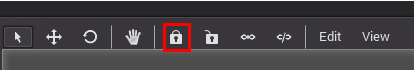
\includegraphics[width=5cm]{img/lvl1-lock.png}
  \end{center}
  \caption{\label{lvl1-lock} Ce petit cadenas peut vous sauver la vie !}
\end{figure}

Vous verrez un cadenas apparaître dans l'onglet \emph{Scene} ainsi que sur dans la vue 2D elle-même, et il signifie que vous ne pouvez pas modifier le \emph{noeud}. Cela parait un peu bizarre de vouloir restreindre ce qu'on peut modifier dans son propre projet, mais il vaut toujours mieux verrouiller ce que vous n'utilisez pas pour le moment. Tant qu'à faire, il vaut mieux éviter de perdre des heures de travail à cause d'un redimenssionnement inopiné qu'on n'avait pas remarqué, n'est-ce pas ?

La dernière chose que nous devons faire, c'est renommer le \emph{noeud}. En effet, sans prendre cette bonne habitude, vous risquez de finir avec une \emph{scène} remplie d'objets nommés \codeintext{Node2D}, et bonne chance pour savoir lequel correspond à quoi.

Pour changer le nom d'un \emph{noeud}, double-cliquez simplement sur son nom dans l'onglet \emph{Scene}, et entrez un nouveau nom. Conseil : choisissez un nom concis, de préférence sans espaces ou caractères spéciaux (un peu comme si vous nommiez une variable). Vous devrez souvent référencer ses noms dans votre code, donc évitez-vous des erreurs inutiles et faites dans la sobriété.

\begin{figure}
  \begin{center}
    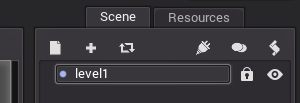
\includegraphics[width=4cm]{img/lvl1-rename.png}
  \end{center}
  \caption{\label{lvl1-rename} Probablement l'habitude la plus importante à attraper...}
\end{figure}

Une fois votre nom choisis, n'oubliez pas d'appuyer sur \emph{enter}, pour valider la saisie. De manière générale, Godot demande souvent de vous que vous validiez ce que vous venez d'entrer. Encore une bonne habitude... Si tout va bien, vous devriez avoir un \emph{noeud} renommé, comme à la figure \ref{lvl1-rename}.

Voilà, ouf, ça y est, notre premier noeud est en place. Que la longueur de cette section ne vous intimide pas : il a fallu aborder beaucoup de concepts en une fois, mais maintenant, l'ensemble pourra être condensé en une phrase à chaque nouveau \emph{noeud} qu'il faudra créer. N'est-ce pas merveilleux ?

En parlant de nouveaux \emph{noeuds}, que diriez-vous d'inclure un personnage à notre embryon de jeu ?

\section{Un peu de \emph{character} (accent british requis)}

Jusqu'ici, beaucoup de blabla pour finalement pas tellement de résultats, n'est-ce pas ? Accrochez vos ceintures, ça va changer !

\subsection{Un nouveau \emph{noeud}}

D'une façon similaire à ce que nous avons vu à la section précédente, nous allons créer un \emph{noeud} qui sera enfant de notre \emph{noeud} \codeintext{level1}. Pour ce faire, sélectionnez \codeintext{level1} avant d'appuyer sur le bouton de création d'un \emph{noeud} (ou sur \codeintext{Ctrl + A}). Cette fois, nous allons utiliser un \emph{noeud} de type \codeintext{AnimatedSprite}, et nous allons le renommer, de façon choquante, en \codeintext{player}. Une fois celà fait, votre onglet \emph{Scene}\footnote{Nous verrons bientôt ce que sont ces fameuses \emph{scènes}...} devrait ressembler à la figure \ref{lvl1-playernode}.

\begin{figure}
  \begin{center}
    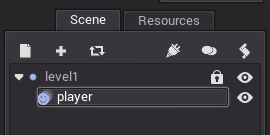
\includegraphics[width=4cm]{img/lvl1-playernode.png}
  \end{center}
  \caption{\label{lvl1-playernode} Attention à ce que \codeintext{player} soit bien enfant de \codeintext{level1}}
\end{figure}

Si vous regardez l'\emph{inspecteur}, vous verrez tout un tas de propriétés regroupées selon qu'elles sont générales ou spécifiques à un certain type de \emph{noeud}. Pour commencer, nous allons dire à Godot quelles images utiliser pour notre personnage.

Pour celà, allons dans l'\emph{inspecteur}, à la propriété \codeintext{Frames} (attention, au pluriel, à ne pas confondre avec \codeintext{Frame} au singulier), et cliquons sur la flèche qui pointe vers le bas. Comme à la figure \ref{lvl1-newframes}, un petit menu va apparaître, et là, contrairement à ce que vous pourriez penser, nous allons ignorer l'option \codeintext{Load} et sélectionner à la place \codeintext{New SpriteFrames}\footnote{Sans entrer dans les détails, l'option \codeintext{Load} ne nous propose pas de charger des images, mais plutôt de charger une ``ressource'', ce que nous allons en fait créer via \codeintext{New SpriteFrames}.}.

\begin{figure}
  \begin{center}
    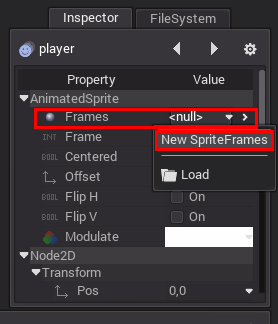
\includegraphics[width=4cm]{img/lvl1-newframes.png}
  \end{center}
  \caption{\label{lvl1-newframes} Comment assigner des images pour notre personnage ? Suivez la flèche vers le bas :D}
\end{figure}

Maintenant que nous avons créé un nouvel objet \codeintext{SpriteFrames}, qui comme son nom l'indique représente un ensemble d'images pour un sprite, nous allons pouvoir les éditer.

Pour se faire, utilisez maintenant la flèche vers la droite (\codeintext{>}) à côté de \codeintext{Frames}, pour faire apparaître l'écran d'édition de nos nouvelles frames. Le changement est assez drastique, comme le montre la figure \ref{lvl1-addframes}, mais nous sommes surtout intéressés par le bouton en haut à gauche qui permet de charger un ou plusieurs fichiers pour les ajouter à nos frames.

\begin{figure}
  \begin{center}
    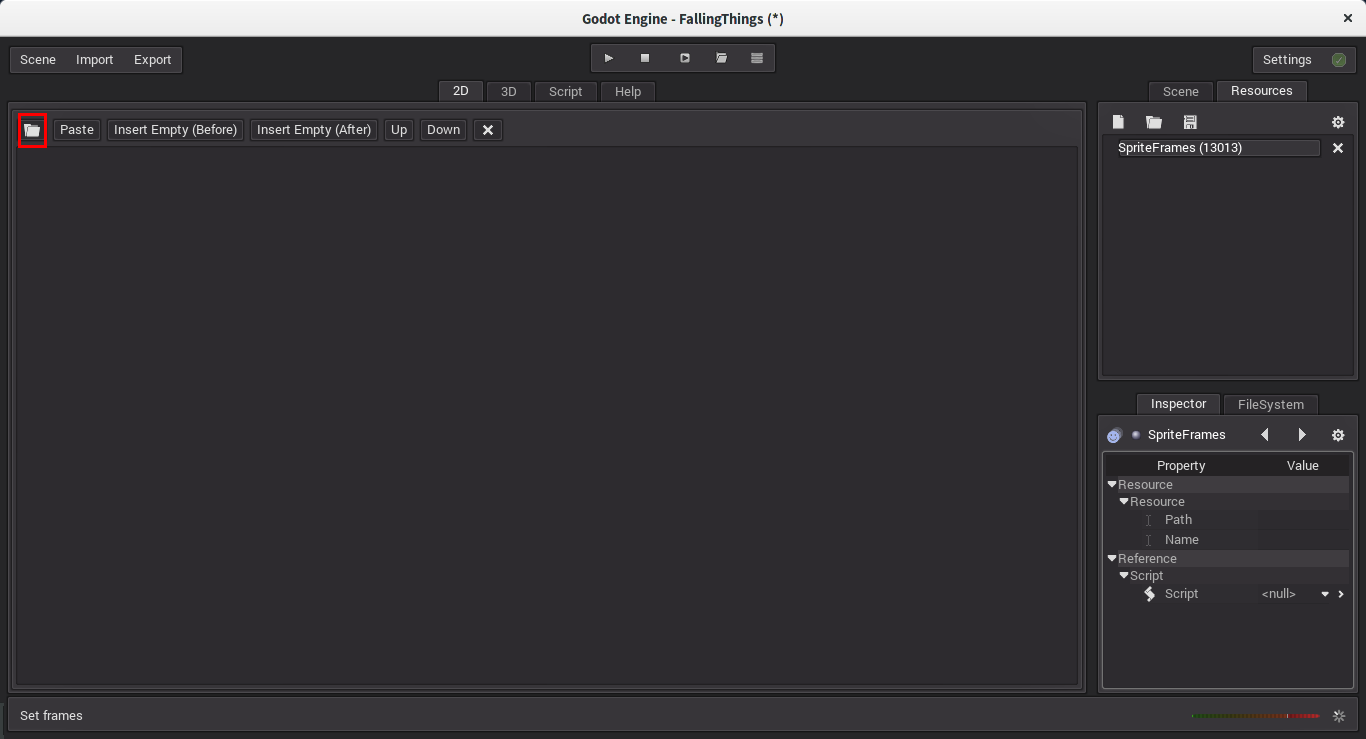
\includegraphics[width=12cm]{img/lvl1-addframes.png}
  \end{center}
  \caption{\label{lvl1-addframes} Un si petit bouton, pour un si grand écran...}
\end{figure}

Avant de charger nos images, un tout petit apparté sur l'organisation de vos projets...

\subsection{Ranger ses dossiers, c'est comme tondre sa pelouse...}

...c'est rébarbatif, ça peut paraître une perte de temps, mais si ce n'est pas fait on se retrouve avec un jardin qui tient plus de la forêt vierge et dont petit à petit on ne sait plus si elle n'abrite pas de dangereux prédateurs là où avant il n'y avait que des bégonias\footnote{Cette métaphore est garantie sans hyperbole (...ou presque).}.

Blague à part, un projet de jeu vidéo va vous demander d'utiliser énormément de types de fichiers différents : effets sonores, musiques, animations, textures, modèles 3D, sprites 2D, shaders, scripts, fichiers XML, la liste est longue. Dès le début du projet, nous vous conseillons donc de veiller à garder votre projet organisé. C'est vraiment essentiel, même si vous êtes pressées par le temps !

Le plus souvent, une organisation par type d'élément est le plus simple. Par exemple, ici, nous allons avoir des sprites. Chaque sprite va avoir plusieurs images pour les différentes étapes de son animation, et donc par conséquent, vous pourriez avoir un dossier \codeintext{sprites} dans le dossier du projet, et mettre un sous-dossier \codeintext{character} dans \codeintext{sprites}, puisque les images fournies pour le personnage sont nommées \codeintext{characterX.png}. Ca n'est pas d'une originalité haletante, mais ça a le mérite d'être clair.

Nous allons, dans la suite du cours, toujours suggérer des noms de dossier pour vous guider dans l'organisation du projet, mais même si vous décidez d'organiser les choses autrement, avoir une méthode pour retrouver vos petits est absolument capital !

Sur ce...

\subsection{Back to work!}

En utilisant le bouton encadré sur la figure \ref{lvl1-addframes}, un sélecteur de fichier va apparaître.

Le sélecteur de fichier va vous permettre de naviguer dans les dossiers du projet pour trouver les images à inclure. Notez que vous ne pouvez aller chercher les images \emph{que} dans le répertoire du projet, il est donc essentiel de copier tout ce dont vous avez besoin dedans. Ici, nous avons créé un dossier \codeintext{sprites/character/} dans lequel les 6 frames sont placées, sous forme de fichier .png.

Pour la petite histoire, nous aurions pû mettre toutes les images en une seule (on appelle ça une \emph{spritesheet}), comme à la figure \ref{lvl1-spritesheet}, mais ici nous avons séparé les images pour travailler plus simplement sans ajouter une complication supplémentaire.

\begin{figure}
  \begin{center}
    
\includegraphics[width=6cm]{img/lvl1-spritesheet.png}
  \end{center}
  \caption{\label{lvl1-spritesheet} Notre magnifique personnage !}
\end{figure}

Une fois que votre sélecteur ressemble à celui de la figure \ref{lvl1-fileselector} (vous pouvez sélectionner plusieurs fichiers en gardant \codeintext{Ctrl} enfoncé, ou en cliquant sur la première, appuyer sur \codeintext{Shift}, et cliquant sur la dernière), appuyez sur \codeintext{Open}.

\begin{figure}
  \begin{center}
    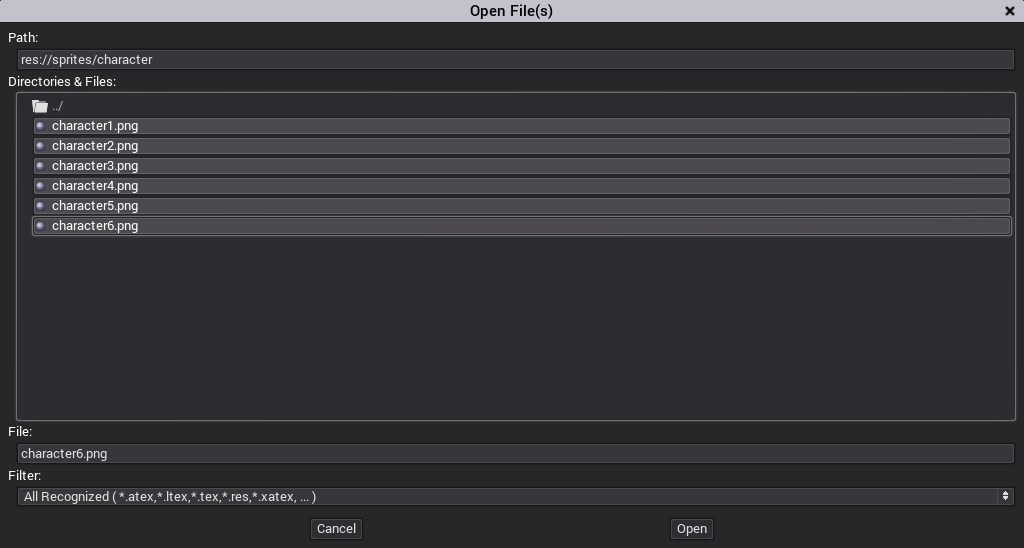
\includegraphics[width=10cm]{img/lvl1-fileselector.png}
  \end{center}
  \caption{\label{lvl1-fileselector} Et voilà nos petites images !}
\end{figure}

Et tadam ! Nos images sont maitnenant à l'intérieur de Godot, prêtes à être utilisées. Après avoir admiré les minuscules previews qui sont affichées, vous pouvez retourner à la scène en cliquant sur la flèche qui pointe vers la gauche dans l'\emph{inspecteur}, ou retourner dans l'onglet \codeintext{Scene} et sélectionner un noeud au hasard. La figure \ref{lvl1-framesadded} est là pour vous guider.

\begin{figure}
  \begin{center}
    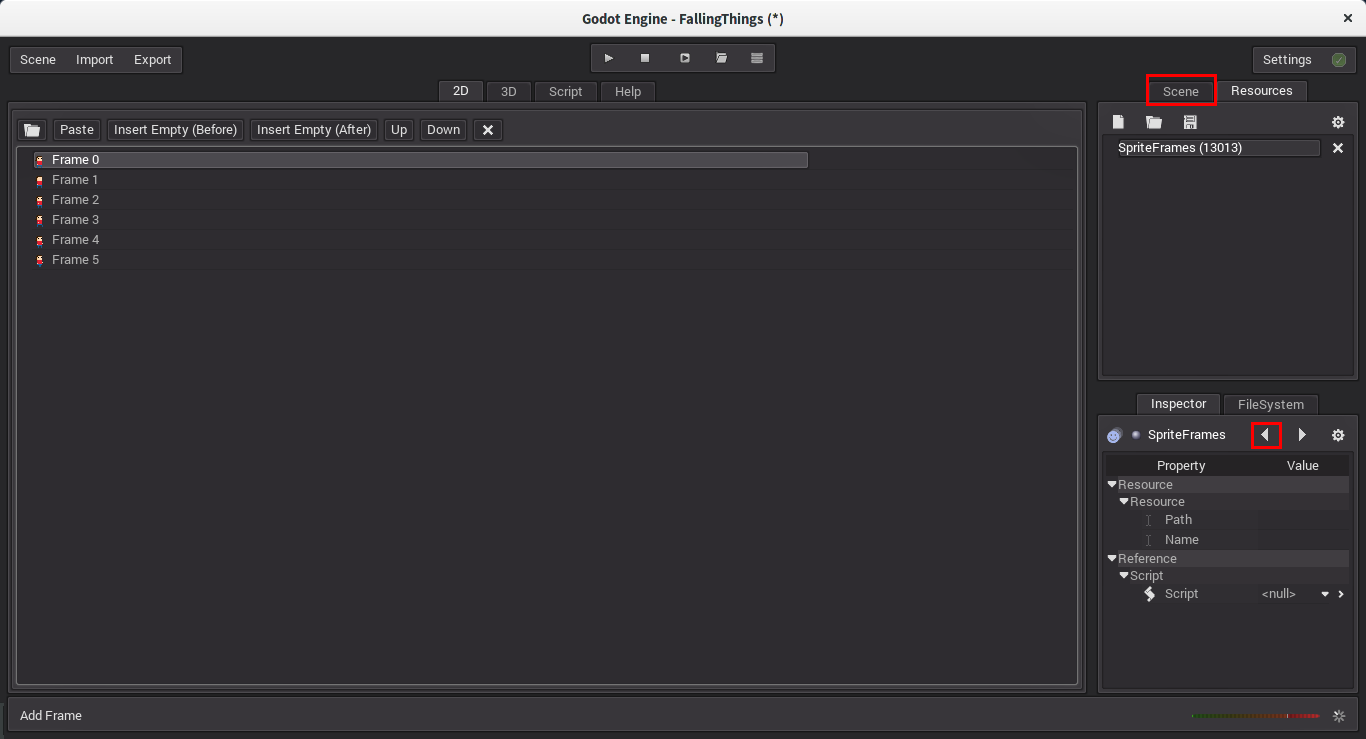
\includegraphics[width=12cm]{img/lvl1-framesadded.png}
  \end{center}
  \caption{\label{lvl1-framesadded} La lumière est au bout du tunnel, notre jeu aura bientôt son premier élément !}
\end{figure}

Une fois de retour sur la scène, vous pourrez zoomer sur votre personnage (via la molette de la souris). Mais là, horreur ! C'est tout flou (voir figure \ref{lvl1-blurred}) ! Est-ce que ça veut dire que le pixel art dans Godot est une cause perdue ?

\begin{figure}
  \begin{center}
    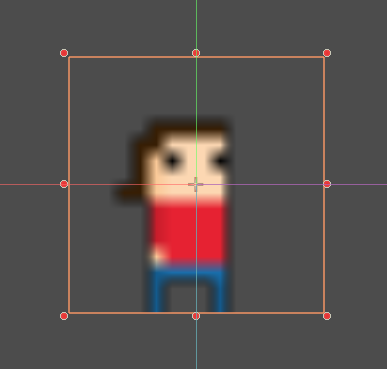
\includegraphics[width=4cm]{img/lvl1-blurred.png}
  \end{center}
  \caption{\label{lvl1-blurred} Tout ça pour ce résultat :( }
\end{figure}

Spoiler alert : non. Tout simplement, par défaut, Godot mets en place une \emph{interpolation}, qui va ``lisser'' les images. C'est souvent une bonne chose, mais dans le cas de pixel art, on veut éviter ça et garder une image bien claire et ``sharp''. Voyons comment faire, et maintenant que notre personnage est dans le jeu, parlons enfin de \emph{scène}.

\section{Mise en \emph{scène}}

Dans cette section, nous allons voir 2 choses : ce qu'est une \emph{scène}, et comment configurer notre projet pour que notre jeu soit affiché correctement.

\subsection{Les \emph{scènes} en Godot}

Dans Godot, une \emph{scène} est simplement une hiérarchie de \emph{noeuds}, sauvegardés en tant que groupe. C'est l'unité de travail principale de l'éditeur de Godot : quand vous éditez votre jeu, vous éditez en fait une  \emph{scène}.

D'un point de vue technique, une \emph{scène} présente les caractéristiques suivantes :

\begin{itemize}
\item Elle contient un certain nombre de \emph{noeuds} organisés en hiérarchie.
\item Elle dispose d'un \emph{noeud} unique, qui sert de racine.
\item Elle peut être sauvegardée ou chargée depuis un fichier.
\item Elle peut être instanciée (plus de détails plus tard là-dessus).
\end{itemize}

Dans un premier temps, vous pouvez approximer une \emph{scène} comme un ``niveau'' de votre jeu, mais nous verrons que le principe est puissant et que nous aurons l'occasion de l'utiliser pour gagner pas mal de temps plus tard.

Il est d'ailleurs grand temps de créer notre première \emph{scène}. En fait, vous êtes en train de l'éditer depuis le début du projet ! Ca peut valoir le coup de la sauvegarder, non ?

Pour se faire, un petit \codeintext{Ctrl + S} (ou bien un détour par le menu \codeintext{Scene > Save Scene}) va vous permettre de sauver votre \emph{scène}. Créez un nouveau sous-dossiers dans votre projet, nommé par exemple \codeintext{scenes}, et nommez votre fichier \codeintext{level1.scn}.

Et voilà, votre travail ne risque plus rien, et nous allons pouvoir maintenant dire à Godot qu'il doit lancer cette \emph{scène} quand vous lancez le jeu. Let's go!

\subsection{Configuration et adieux au flou}

Godot vous permet de configurer pas mal de choses dans votre projet, et nous allons en tirer profit pour paramétrer notre projet, du moins pour faire le strict nécessaire. Si vous ouvrez le menu \codeintext{Scene > Project Settings}, une fenêtre avec plein d'options va apparaître.

La première option que nous cherchons est l'option qui met en route l'interpolation responsable du flou de notre pauvre sprite. Il s'agit de l'option \codeintext{filter} de la catégorie \codeintext{image\_loader}. Sur la ligne, il y a 2 cases à cocher. Décochez celle de droite (qui est la valeur de l'option), et normalement, comme à la figure \ref{lvl1-filtersetting}, celle de gauche va se cocher automatiquement. C'est normal, la case à cocher de gauche indique simplement que l'option a été modifiée par rapport à sa valeur par défaut. Si vous ne voulez pas prendre en compte un changement, vous pouvez simplement la décocher avant de fermer la fenêtre, et l'option reprendra sa valeur par défaut.

\begin{figure}
  \begin{center}
    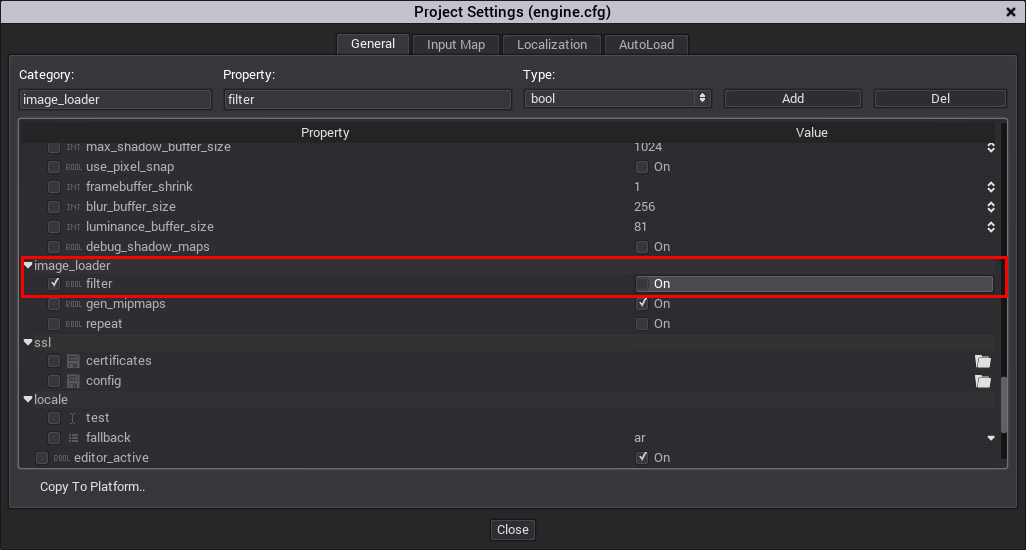
\includegraphics[width=10cm]{img/lvl1-filtersetting.png}
  \end{center}
  \caption{\label{lvl1-filtersetting} Attention à la confusion dans les cases à cocher !}
\end{figure}

Dans la même catégorie, désactivez aussi l'option \codeintext{gen\_mipmaps}. Grâce à cette option, Godot ne va pas tenter de créer des version ``optimisées'' de nos images, ce qui pourrait poser des problèmes du même genre que le filtre.

L'autre option qui nous intéresse est dans la catégorie \codeintext{application}, et se nomme \codeintext{main\_scene}. Comme le nom l'indique\footnote{Avec le nombre de fois où on écrit ça, on voit l'importance de nommer les choses correctement, non ?}, il s'agit de la \emph{scène} principale du jeu. C'est celle qui sera chargée au démarrage de Godot, et qui sera lancée en premier lieu par le jeu final.

Sélectionnez votre \emph{scène}, et cliquez sur \codeintext{Close} pour valider vos choix.

Vous verrez que le sprite est toujours flou ! Pas de panique, c'est normal. Fermez Godot et relancez-le, pour que cette option soit prise en compte.

Si tout a été fait correctement, votre projet sera ouvert, la \emph{scène} chargée, et votre sprite sera affiché dans toute sa splendeur. C'est le cas ? Congratulations !

\section{Et que ça bouge !}

Il est temps de passer à l'animation de notre personnage. Dans Godot, il existe un noeud précisemment prévu pour ça, nommé \codeintext{AnimationPlayer}. Maintenant, vous devriez savoir comment créer un \emph{noeud} de ce type, attaché à notre \emph{noeud} \codeintext{player}. Renommez-le en \codeintext{animator}, et vous constaterez un changement quand \codeintext{animator} est sélectionner : l'interface se modifie pour faire apparaître la barre d'animation ! Celà devrait ressembler à la figure \ref{lvl1-animbar}.

\begin{figure}
  \begin{center}
    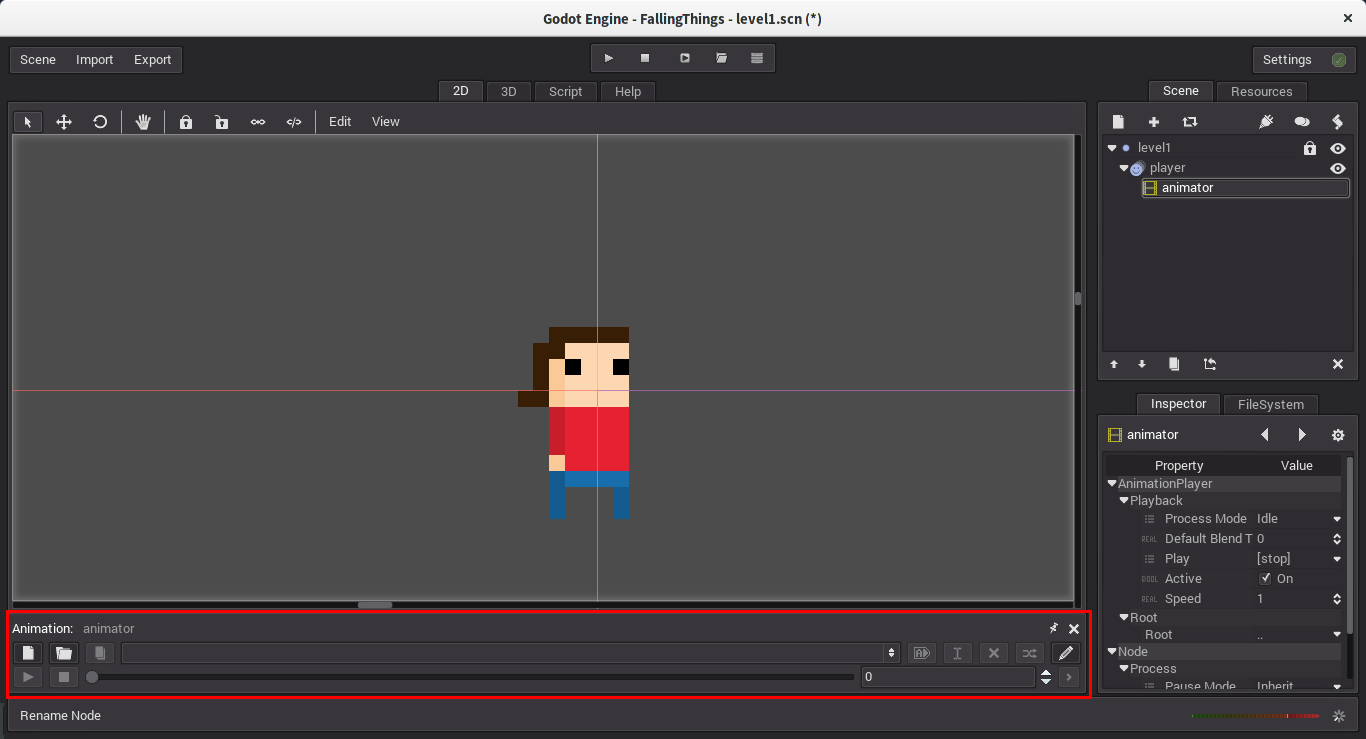
\includegraphics[width=12cm]{img/lvl1-animbar.png}
  \end{center}
  \caption{\label{lvl1-animbar} La barre qui va donner vie à notre personnage.}
\end{figure}

Passons à la création de notre première animation, l'animation de notre personnage au repos. Pour ce faire, cliquez sur le bouton de création d'une nouvelle animation et nommez-là par exemple \codeintext{idle} (repos), comme à la figure \ref{lvl1-createidle}.

\begin{figure}
  \begin{center}
    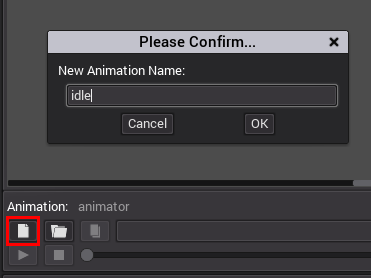
\includegraphics[width=5cm]{img/lvl1-createidle.png}
  \end{center}
  \caption{\label{lvl1-createidle} Création d'une nouvelle animation.}
\end{figure}

Une fois celà fait, éditez l'animation via le bouton représentant un crayon, à droite de la barre d'animation, comme à la figure \ref{lvl1-animeditbutton}.

\begin{figure}
  \begin{center}
    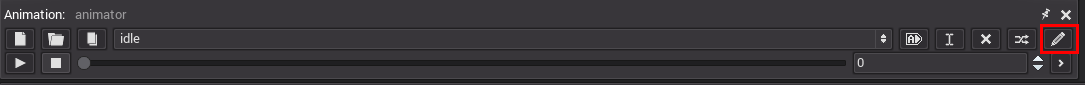
\includegraphics[width=12cm]{img/lvl1-animeditbutton.png}
  \end{center}
  \caption{\label{lvl1-animeditbutton} Le bouton d'édition des animations.}
\end{figure}

La barre d'animation va s'étendre, et vous présenter une ligne du temps pour l'instant vide. Vous allez pouvoir ajouter des pistes à cette ligne du temps, qui vont correspondre à différentes propriétés de vos \emph{noeuds} que vous allez pouvoir animer. Vous pourrez constater que l'\emph{inspecteur} affiche maintenant des clefs à côté de chaque propriété. Apppuyer sur une de ces clefs va créer une \emph{keyframe}, c'est à dire stocker la valeur d'une propriété à un moment donné de l'animation.

Sélectionnez le \codeintext{player} et cliquez sur la petite clef à droite de \codeintext{Frame} (au singulier !) dans l'\emph{inspecteur}. Acceptez que Godot crée une nouvelle piste, comme sur la figure \ref{lvl1-animnewtrack}.

\begin{figure}
  \begin{center}
    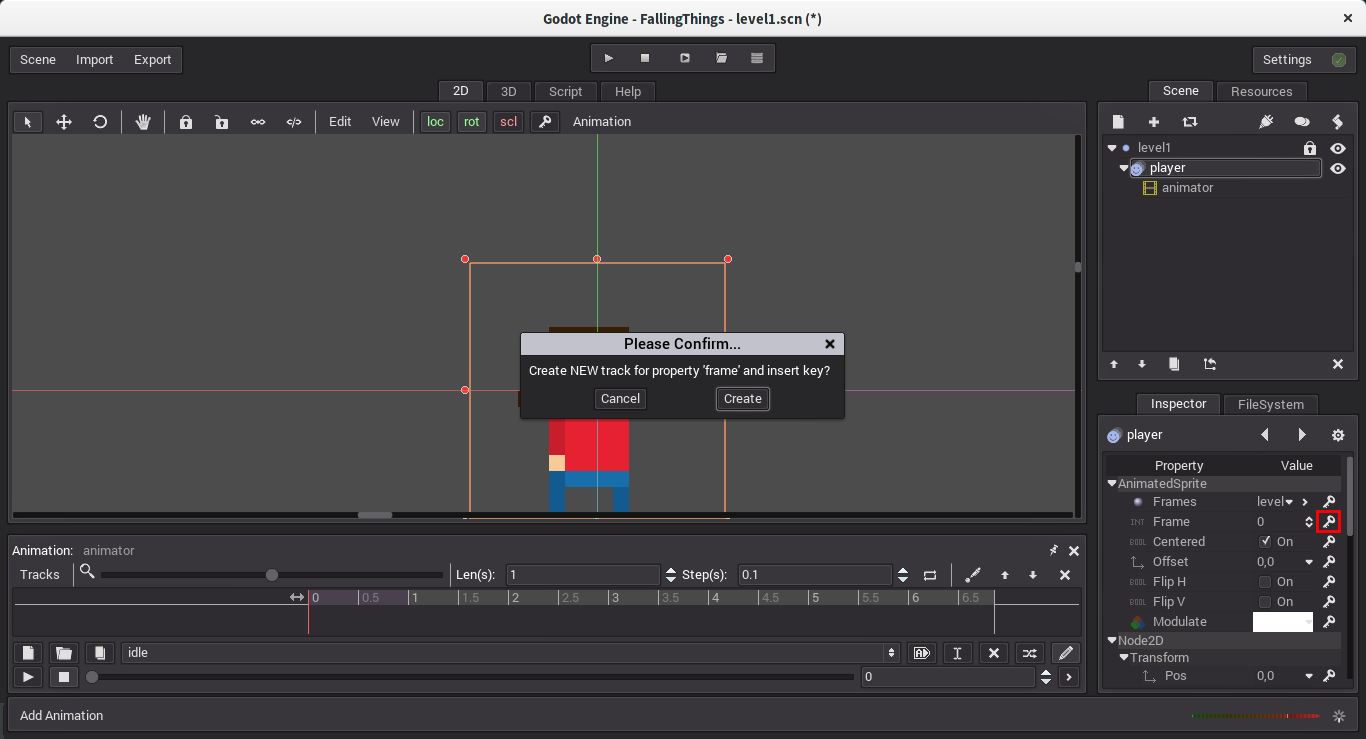
\includegraphics[width=12cm]{img/lvl1-animnewtrack.png}
  \end{center}
  \caption{\label{lvl1-animnewtrack} Godot vous demande si vous voulez vraiment créer une nouvelle piste dans votre animation.}
\end{figure}

La façon dont nous allons animer notre personnage est dire à Godot quand il doit changer de frame, via la ligne du temps. Le slider dans la partie inférieure de la barre d'animation permet de se déplacer sur la durée de l'animation. Nous allons faire en sorte que le personnage cligne des yeux. Il a suffit de 2 frames pour ça, une avec les yeux ouvertes, une avec les yeux fermés. Un clignement d'oeil étant très court, nous allons effectuer le changement de frame pendant un court laps de temps. Avancez jusqu'à être à 0.9 secondes, changez la propriété \codeintext{Frame} à 1 dans l'\emph{inspecteur}, et appuyez sur la clef, comme montré à la figure \ref{lvl1-animaddkeyframe}.

\begin{figure}
  \begin{center}
    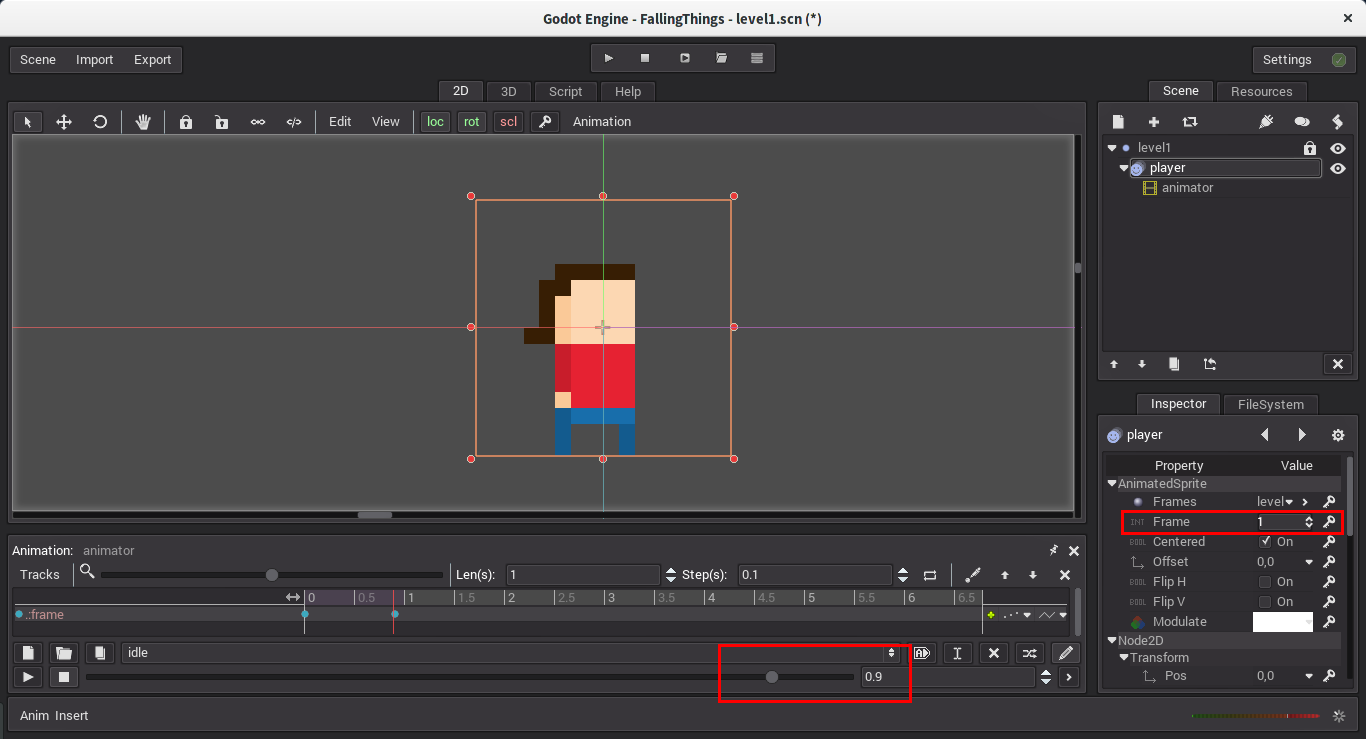
\includegraphics[width=12cm]{img/lvl1-animaddkeyframe.png}
  \end{center}
  \caption{\label{lvl1-animaddkeyframe} Le résultat une fois la keyframe ajoutée.}
\end{figure}

Répétez le processus pour ajouter une keyframe à la fin de l'animation (position 1.0 sur la timeline).

si vous appuyez sur play (dans la barre d'animation, pas au-dessus), vous pourrez voir votre personnage cligner des yeux, et puis les garder ouverts, au risque de s'assécher les globes occulaires. C'est simplement parce que l'animation n'est pas en mode ``boucle''. Pour remédier à ça, utilisez le bouton idoine renseigné à la figure \ref{lvl1-animloop}. Mieux, mais un peu robotique, non ?

\begin{figure}
  \begin{center}
    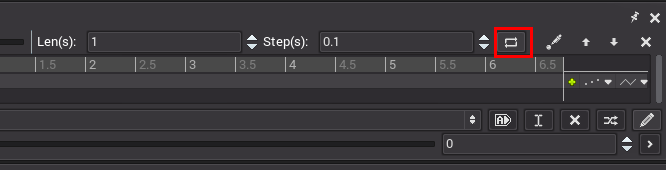
\includegraphics[width=5cm]{img/lvl1-animloop.png}
  \end{center}
  \caption{\label{lvl1-animloop} Sauvons les yeux du pauvre sprite.}
\end{figure}

Pour éviter l'effet un peu perturbant de la boucle régulière, il suffit de rajouter quelques clignements espacés différement. Sur la figure \ref{lvl1-animloop}, vous pouvez voir un paramètre \codeintext{Len(s)}. Celui-ci contrôle la longueur de l'animation. Augmentez-le (à 3 ou 5 par exemple), et utilisez les étapes précédentes pour ajouter quelques clignements supplémentaires par-ci, par-là, jusqu'à ce que l'animation semble plus naturelle.

Nous avons utilisé les 2 premières images, mais il y en avait 4 autres. Pour ne pas les gaspillez, créez une nouvelle animation, nommée \codeintext{walk}, avec les 4 frames restantes, espacées par exemple chacune de 0.2 secondes. C'est exactement le même principle que pour l'animation \codeintext{idle}, donc ça devrait aller !

Une fois que votre personnage est capable de marcher\footnote{Rappel en passant, n'oubliez pas de sauvegarder de temps en temps !}, nous allons le placer dans un environnement un peu rigolo, avant de passer au code.

\section{Décor, Caméra, Action !}

En utilisant ce que nous avons vu plus haut, nous allons rajouter le décor, et par la même occasion mettre quelques options à jour pour notre cas particulier (un jeu 2D en pixel art).

\subsection{Monter le décor}

Avant toute chose, nous allons configurer notre éditeur pour qu'il aligne les noeuds sur une grille de pixels exacte. Sans ça, malgré tous vos vaillants efforts vous aurez sûrement des problèmes d'alignement, même s'ils seront indétectables à l'oeil nu. Pour aligner notre jeu au pixel près, utilisez le menu \codeintext{Edit}, comme le montre la figure \ref{lvl1-pixelsnap}.

\begin{figure}
  \begin{center}
    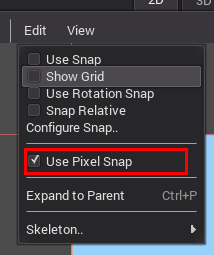
\includegraphics[width=4cm]{img/lvl1-pixelsnap.png}
  \end{center}
  \caption{\label{lvl1-pixelsnap} Alignez sur une grille, alignez sur les pixels, alignez jusqu'à ce que tout soit aligné !}
\end{figure}

Une fois ceci fait, ajoutez un \codeintext{Node2D} (nommé par exemple \codeintext{environment}) vide pour contenir le décor, et 2 \codeintext{AnimatedSprite} pour le ciel et le sol respectivement, enfants de \codeintext{environment}. Ajoutez une frame comme pour le personnage, et vous devriez finir avec une situation similaire à la figure \ref{lvl1-centered}. Notez que l'ordre des \emph{noeuds} dans la \emph{scène} est important. Toute chose étant égale par ailleurs, Godot va les afficher dans l'ordre où il les rencontre. Nous aurons l'occasion de voir comment changer ça, mais pour l'instant mettez simplement \codeintext{environment} au-dessus de \codeintext{player} pour que tout soit affiché correctement.

\begin{figure}
  \begin{center}
    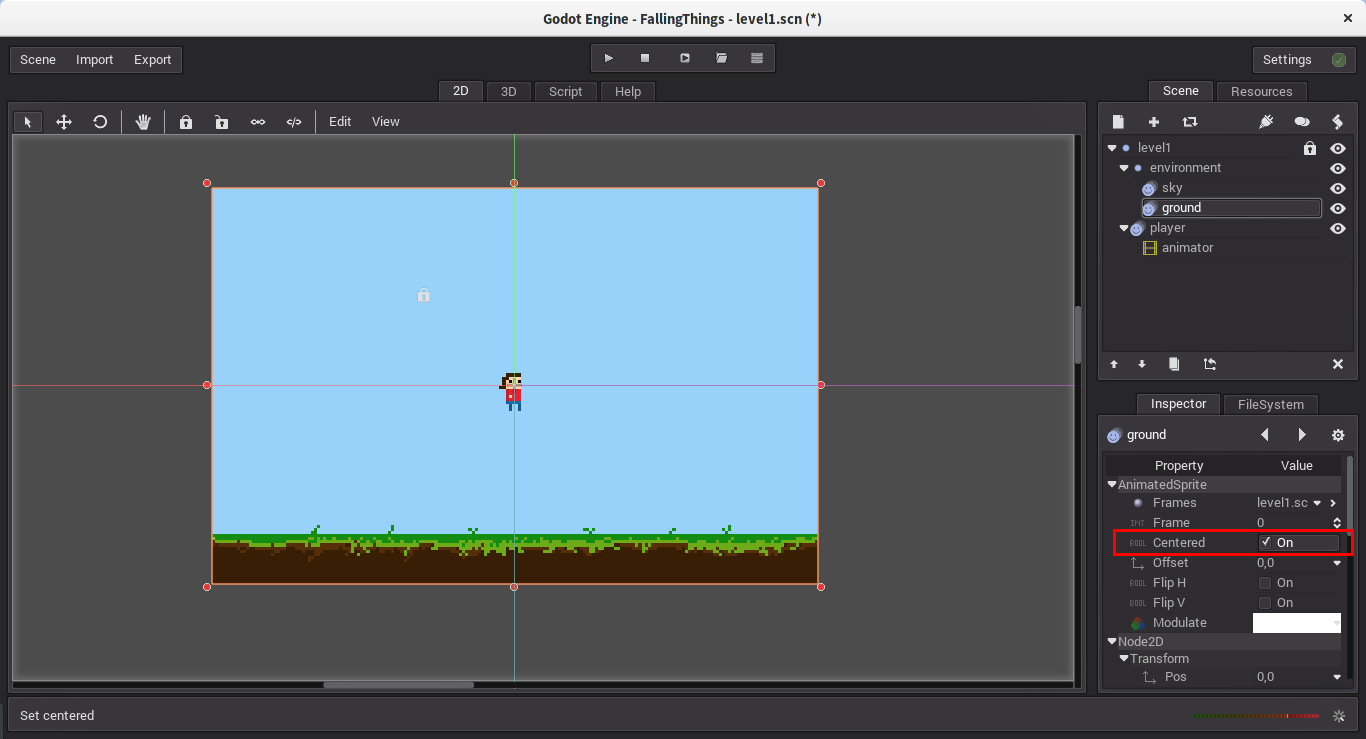
\includegraphics[width=12cm]{img/lvl1-centered.png}
  \end{center}
  \caption{\label{lvl1-centered} Le décor, une fois importé, et comment éviter qu'il soit centré.}
\end{figure}

L'autre point que la figure \ref{lvl1-centered} met en évidence est la propriété \codeintext{Centered}. En effet, par défaut, Godot place l'origine de toutes les images au centre de celles-ci. Si vous travaillez comme nous le faisons ici en pixel art, vous pourriez avoir des surprises si vos images ont une dimension impaire (l'origine serait ``au milieu'' d'un pixel). Ici ce n'est pas le cas, mais par précaution...

Décochez la propriété, et vous verrez que les décors se déplaceront pour, mettre leur coin supérieur gauche à l'origine des axes. C'est parce que Godot prend maintenant ce coin comme origine au lieu du centre de l'image. N'oubliez pas d'aussi décocher \codeintext{Centered} sur \codeintext{player}.

Vous pouvez maintenant déplacer le personnage pour le mettre au niveau du sol. Et une fois qu'il est placé à votre convenance, vous allez pouvoir lancer le jeu ! Cliquez sur Play tout en haut de l'écran et constatez que...

\begin{enumerate}
\item C'est tout petit.
\item Le personnage n'a pas l'air de cligner des yeux.
\end{enumerate}

Nous allons bien entendu résoudre ces 2 problèmes...

\subsection{Allumer les caméras}

Quand vous avez lancé le jeu, Godot a affiché le jeu à sa résolution ``native''. Comme nous travaillons en basse résolution, le résultat est que l'affichage est vraiment minuscule.

Pour remédier à ce petit\footnote{C'est le cas de le dire!} soucis, nous allons créer une caméra, et l'utiliser pour zoomer l'ensemble du niveau. Le \emph{noeud} qui sert à celà est \codeintext{Camera2D}, et vous pouvez la renommer en \codeintext{camera}, nous n'en aurons qu'une.

Il va vous falloir éditer quelques propriétés de la caméra :

\begin{description}
\item[\codeintext{Current} :] Cochez la case.
\item[\codeintext{Zoom} :] Mettez 0.25 pour les 2. C'est un peu contre-intuitif, mais pour zoomer 4x, il faut indiquer 0.25 (un quart) ici...
\end{description}

Ensuite, redimensionnez le rectangle de la caméra pour qu'elle prenne tout notre décor. Si vous lancez le jeu à ce stade, c'est mieux, mais pas encore génial. Pour peaufiner ça, allez dans les options du projet et modifiez-les comme suit :

\begin{description}
\item[\codeintext{width} :] 784, à savoir 196 multiplié par 4.
\item[\codeintext{height} :] 512, ou encore 128 multiplié par 4.
\item[\codeintext{resizable} :] Décochez la case, pas besoin de laisser le joueur redimensionner la fenêtre dans notre cas.
\end{description}

Une fois le tout terminé, si vous lancez le jeu, la magie devrait opérer, et le jeu avoir le look de la figure \ref{lvl1-gamerun}.

\begin{figure}
  \begin{center}
    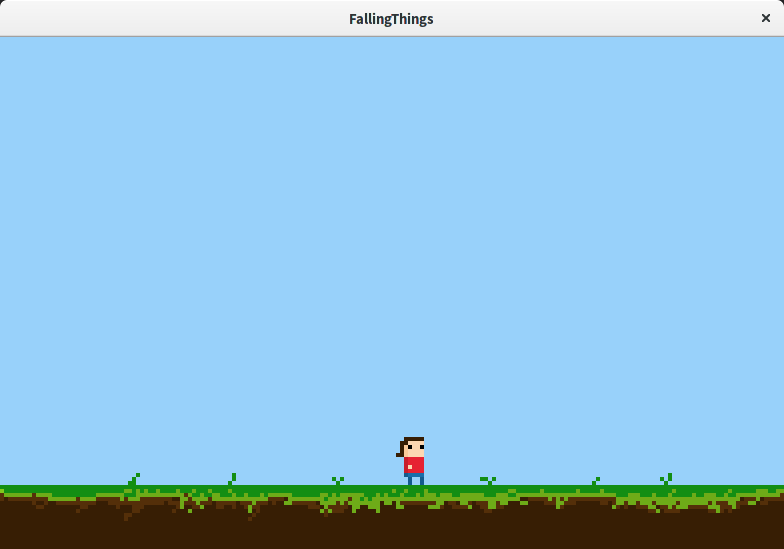
\includegraphics[width=8cm]{img/lvl1-gamerun.png}
  \end{center}
  \caption{\label{lvl1-gamerun} C'est qu'on dirait presque un jeu !}
\end{figure}

C'est donc le problème 1 résolu. Passons au problème 2.

\subsection{Rendre la vie au personnage}

Notre problème est ici heureusement beaucoup plus simple que le précédent. Il s'agit simplement de faire savoir à Godot que, dès le lancement du jeu, certaines animations doivent être actives.

En sélectionnant ce bon vieil \codeintext{animator}, et en faisant apparaître la barre d'animation, vous pouvez simplement appuyer sur le bouton \codeintext{AutoplayOnLoad}, comme indiqué à la figure \ref{lvl1-autoplay}.


\begin{figure}
  \begin{center}
    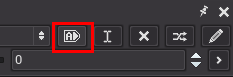
\includegraphics[width=4cm]{img/lvl1-autoplay.png}
  \end{center}
  \caption{\label{lvl1-autoplay} Tout est prévu ! (Sauf faire le café, mais c'est sûrement prévu...)}
\end{figure}

Si vous lancez le jeu à ce stade, c'est bon, notre personnage ne devrait plus être en compétition pour le concours du plus long regard, et s'être mis à cligner des yeux.

N'oubliez pas de verrouillez les noeuds du décor une fois qu'ils sont bien placés, ainsi que la caméra ! Pas de raison de perdre du temps suite à une mauvaise manipulation plus tard...

Notez qu'avec tout ça, vous pourriez facilement ajouter des décors animés et autres fioritures qui rendraient le jeu plus dynamique. Malheureusement, nous n'avons pas le temps pour faire ça maintenant, et devons à la place passer sur un volet probablement un peu plus intimidant.

Il est temps de se mettre à coder.

\section{Les mains dans le cambouis, ou comment faire courir notre personnage}

Fini de rire, jusqu'ici nous nous en sommes tirés sans devoir écrire de code, mais c'est fini. 

Mais, à toute chose malheur est bon, et au moins le langage que Godot emploie, le GDScript, est extrêmement proche du Python. Il y a quelques variantes, mais la syntaxe du langage est presque totalement équivalente à du Python.

Avant de nous lancer à corps perdu dans l'écriture du code qui nous permettra de faire bouger notre personnage, passons en revue ce que nous allons devoir faire.

\begin{enumerate}
\item Tant que le joueur appuye sur la flèche de gauche, le personnage doit avancer vers la gauche.
\item Tant que le joueur appuye sur la flèche de droite, le personnage doit avancer vers la droite.
\item Si le joueur relâche les touches, le personnage doit être stationnaire.
\item Si le personnage bouge, il doit jouer son animation \codeintext{walk}.
\item Si le personnage ne bouge pas, il doit jouer son animation \codeintext{idle}.
\item Le personnage doit resté confiné dans une zone au centre de l'écran.
\end{enumerate}

Tout ça fait pas mal de boulot. Mais en prenant les choses une à une, on devrait s'en sortir.

Malgré l'aspect simple du jeu que nous sommes en train de créer, nous allons quand même nous poser la question de l'organisation de notre code. Pour tout ce qui concerne le personnage, l'examen de la liste ci-dessus rend apparent une organisation possible : Certaines tâches intéragissent avec les contrôles (1-3), tandis que d'autres se rapportent au sprite du personnage lui-même (4-6).

Nous allons donc séparer notre code de la même manière. Nous allons commencer par écrire un script interagissant avec le clavier via les fonctions fournies par Godot, et ensuite nous écrirons un script que nous attacherons au sprite lui-même.

\subsection{Gauche, droite, gauche, droite !}

Il est presque temps d'écrire nos premières lignes de GDScript, mais pour ce faire, encore faut-il savoir où les écrire.

Nous allons utiliser l'interface de Godot afin de créer un fichier \codeintext{.gd} (l'extension utilisée pour le GDScript). Il faut cependant savoir que dans Godot, contrairement à d'autres moteurs de jeu, il n'est pas possible d'attacher plusieurs scripts à un même \emph{noeud}, et que puisque nous avons décidé de séparer notre code en deux scripts, il va falloir créer un nouveau \emph{noeud} pour acceuillir le code de ce que nous appèlerons le \emph{controlleur}.

Créez un \emph{noeud} de type \codeintext{Node}, enfant de \codeintext{player}, et renommez-le en, par exemple, \codeintext{playercontroller}.

Ensuite, en vous guidant avec la figure \ref{lvl1-playercontroller}, cliquez sur le bouton de création d'un nouveau script, en faisant attention à bien avoir sélectionné le \emph{noeud} \codeintext{playercontroller} auparavant.

\begin{figure}
  \begin{center}
    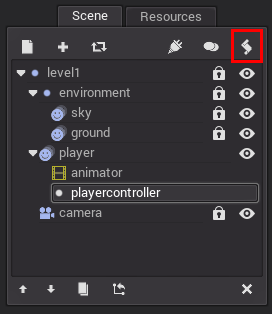
\includegraphics[width=4cm]{img/lvl1-playercontroller.png}
  \end{center}
  \caption{\label{lvl1-playercontroller} L'habitat naturel de notre premier script.}
\end{figure}

En cliquant sur ledit bouton, une boite de dialogue comme celle de la figure \ref{lvl1-createscript} va apparaître.

\begin{figure}
  \begin{center}
    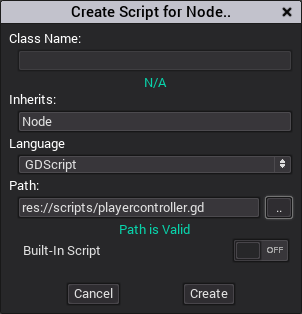
\includegraphics[width=6cm]{img/lvl1-createscript.png}
  \end{center}
  \caption{\label{lvl1-createscript} Création d'un nouveau script. Le nom de classe n'est pas utile pour le moment.}
\end{figure}

La seule chose dont vous devez vous soucier est le nom de fichier. Pour l'instant nous n'utiliserons pas de classe, et donc à vous de, comme d'habitude, créer un dossier et choisir un nom de fichier qui sont clairs et organisés. Ici, nous avons créé un dossier \codeintext{scripts}, et \codeintext{playercontroller.gd} comme nom de script.

Une fois le script créé, vous vous retrouverez dans l'onglet \codeintext{Script} de Godot qui vous permettra donc d'éditer le code de vos scripts. Comme à la figure \ref{lvl1-codeeditor}, vous verrez que Godot a même gentiment écrit le début du script pour vous !

\begin{figure}
  \begin{center}
    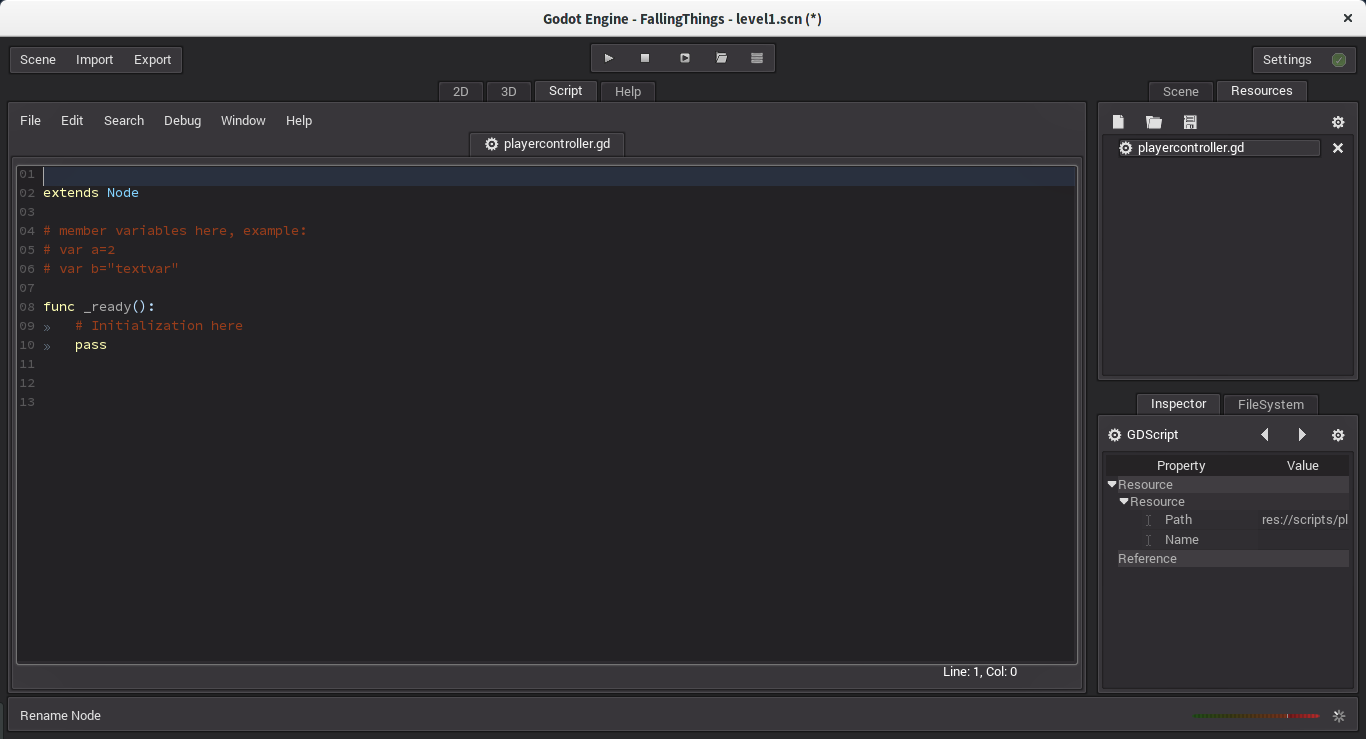
\includegraphics[width=12cm]{img/lvl1-codeeditor.png}
  \end{center}
  \caption{\label{lvl1-codeeditor} Godot vient avec son propre éditeur de code, n'est-ce pas magnifique ?}
\end{figure}

Dans le code écrit par Godot, vous pouvez voir certaines choses familières, et d'autres qui le sont moins. Les points identiques sont :

\begin{itemize}
\item L'utilisation de \codeintext{pass} pour ne rien faire.
\item Les parenthèses et le deux points après les définitions de fonctions.
\item L'utilisation de l'indentation pour délimiter les fonctions.
\item La façon de dénoter les commentaires.
\item L'affectation d'un entier ou d'une chaine de caractères via un signe égal.
\end{itemize}

C'est loin d'être l'ensemble, mais celà vous donne au moins de quoi vous raccrocher. A l'inverse, les points différents sont :

\begin{itemize}
\item L'utilisation de \codeintext{func} au lieu de \codeintext{def}.
\item L'utilisation de \codeintext{var} pour définir une variable.
\item L'utilisation de \codeintext{extends}, qui fonctionne un peu comme \codeintext{import} mais pas vraiment.
\end{itemize}

Nous n'allons pas (du moins pas tout de suite) nous intéresser à \codeintext{extends}, mais les 2 autres, vous allez les rencontrer tout le temps, et donc 5 minutes d'explications valent la peine.

\codeintext{func} est véritablement un remplacement pour \codeintext{def}, et c'est tout. Si vous avez des erreurs, souvenez-vous de vérifier que vous n'avez pas simplement laisser un \codeintext{def} traîner...

L'utilisation de \codeintext{var} est par contre une vraie différence. En Python, vous pouvez créer des variables comme bon vous semble. Ici, Godot va vous demander de créer les variables explicitement en utilisant \codeintext{var}. C'est regrettable, mais c'est ainsi !

Passons au code en lui-même. Pour l'instant, Godot vous fournit simplement une fonction vide, nommée \codeintext{\_ready()}, qui sera appelée au chargement dans l'objet, et une fois seulement. Dans Godot, les \emph{noeuds} proposent de nombreuses fonctions, et nous allons en utiliser une autre.

Modifiez votre script votre script de la façon suivante, afin de détecter les touches du claviers.

\begin{lstlisting}
extends Node

func _ready():
    set_process(true)

func _process(deltatime):
    if Input.is_key_pressed(KEY_LEFT):
        print("A gauche")
    if Input.is_key_pressed(KEY_RIGHT):
        print("A droite")
\end{lstlisting}

Une fois les modifications faites, assurons-nous que le code fait bien ce que nous voulons en lançant le jeu et en testant les touches gauche et droite du clavier. Normalement, comme sur la figure \ref{lvl1-output}, vous devriez voir la sortie de votre jeu dans la fenêtre présentée par Godot. 

\begin{figure}
  \begin{center}
    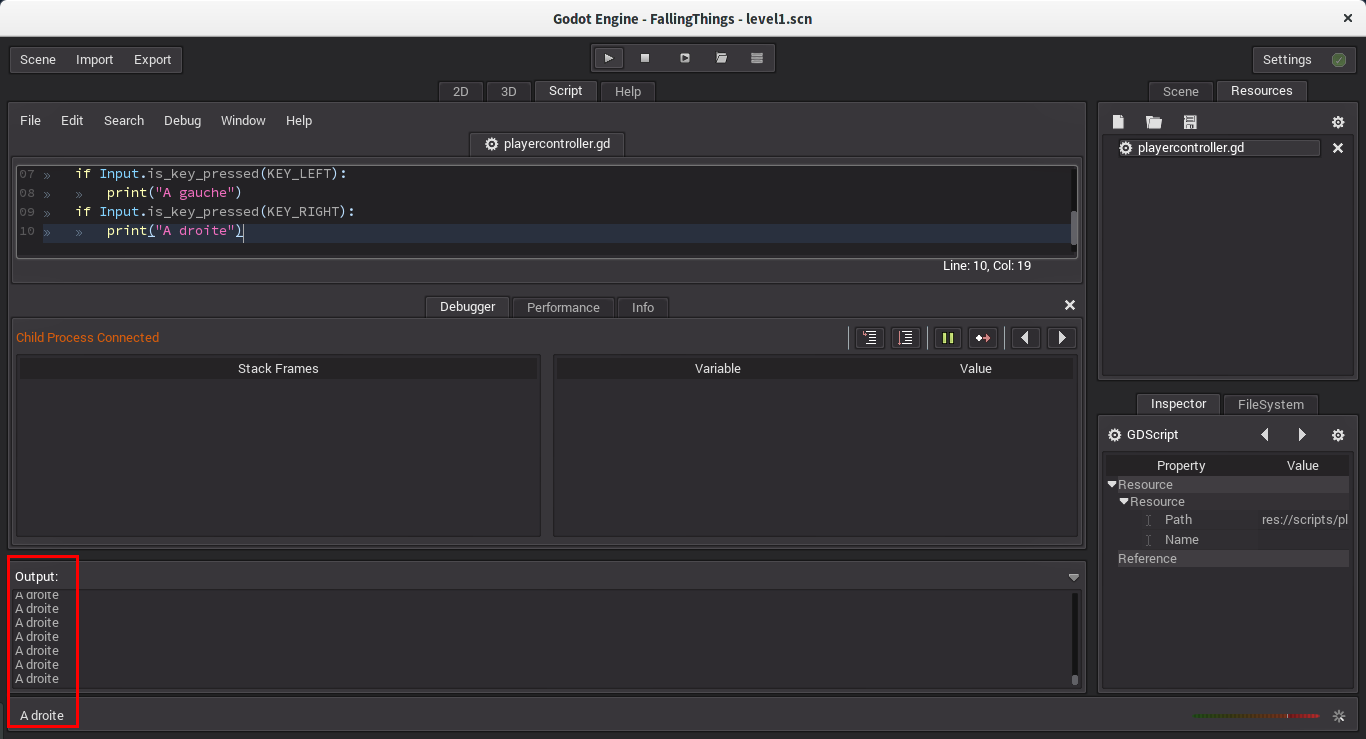
\includegraphics[width=12cm]{img/lvl1-output.png}
  \end{center}
  \caption{\label{lvl1-output} Le debugger de Godot, qui vous montre ici la sortie de votre jeu.}
\end{figure}

Avant d'aller plus loin, examinons le code de l'extrait ci-dessus.

La principale difficulté est l'utilisation d'une nouvelle fonction, \codeintext{\_process(deltatime)}, et ce qu'il se passe dans \codeintext{\_ready()}.

\codeintext{\_process} est l'une des fonctions fournies par Godot. Vous pouvez voir sa documentation en pressant \codeintext{Shift + F1} quand votre curseur est dessus. Mais, pour tout vous dire, il s'agit s'implement d'une fonction qui est appelée à chaque frame du jeu pour chaque \emph{noeud} dont le script est marqué comme voulant être traité.

Et c'est bien celà qui est fait dans la fonction \codeintext{\_ready()} : en faisant appel à \codeintext{set\_process(true)}, vous dites à Godot ``oui, je veux que la fonction \codeintext{\_process} de ce script soit appelée à chaque frame''.

Les conditions des \codeintext{if} devraient être assez familière après le cours de Python. Cependant, il est possible de faire un peu mieux en Godot, grâce aux actions.

\subsection{Actions et réactions}

Si vous ouvrez la fenêtre des paramètres du projet, vous verrez qu'il y a plusieurs onglets. Dans l'onglet \codeintext{Input Map}, vous trouverez l'endroit où vous pourrez définir des actions à assigner aux boutons et touches de clavier que vous désirerez. C'est un mécanisme bien pratique, vous allez voir.

Par défaut, comme le montre la figure \ref{lvl1-actions}, il y a beaucoup d'actions définies, nous allons donc commencer par toutes les supprimer.

\begin{figure}
  \begin{center}
    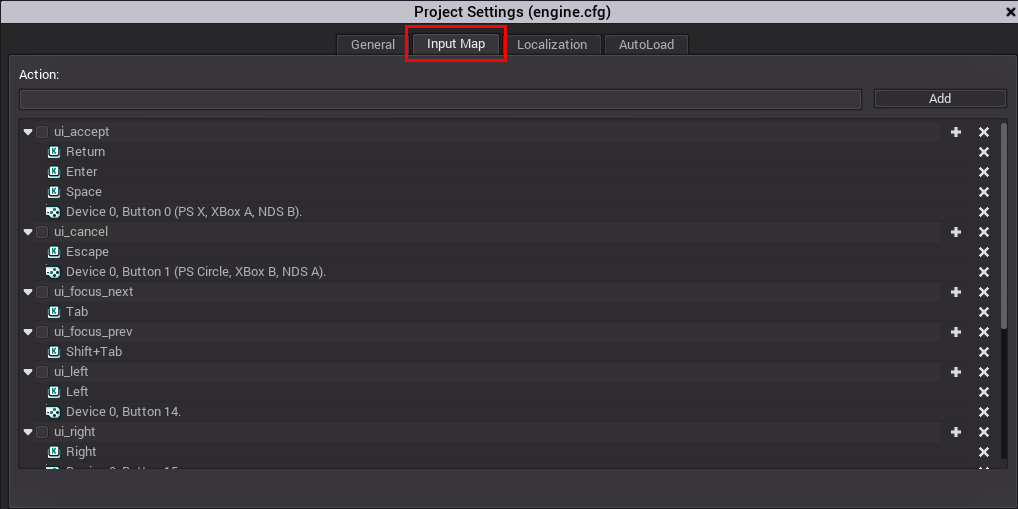
\includegraphics[width=8cm]{img/lvl1-actions.png}
  \end{center}
  \caption{\label{lvl1-actions} Les actions par défaut, beaucoup trop pour nous !}
\end{figure}

Une fois la fenêtre vidée, ajoutez deux nouvelles actions, \codeintext{player\_left} et \codeintext{player\_right}, et assignez-leur une ou deux touches du clavier. La liste des actions devrait maintenant ressembler à celle de la figure \ref{lvl1-ouractions}.

\begin{figure}
  \begin{center}
    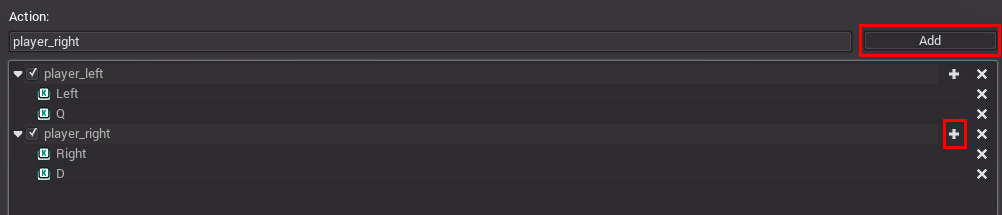
\includegraphics[width=8cm]{img/lvl1-ouractions.png}
  \end{center}
  \caption{\label{lvl1-ouractions} Nos actions, voilà qui est mieux !}
\end{figure}

Il ne reste plus qu'à retourner dans notre script, et modifier quelque peut le code.

Au lieu de

\begin{lstlisting}
Input.is_key_pressed(KEY_LEFT)
\end{lstlisting}

vous pouvez maintenant utiliser les actions comme suit :

\begin{lstlisting}
Input.is_action_pressed("player_left")
\end{lstlisting}

Le changement peut paraître anodin, mais le jour où vous voudrez accepter un contrôleur console en plus du clavier, vous serez bien contentes de pouvoir le faire simplement !

Nous obtenons donc maintenant bien une réaction de Godot quand nous appuyons sur certaines touches du clavier. Il est temps de passer de l'autre côté de la barrière et s'occuper du personnage.

\subsection{Réanimation}

Le but ici va être de faire jouer les bonnes animations au bon moment, et faire bouger le sprite.

Nous allons créer le script ensemble (et l'attacher à \codeintext{player}), mais voici la liste des éléments dont vous aurez besoin.

\begin{itemize}
\item Si, avant la première fonction, vous utilisez \codeintext{export var ...}, vous pourrez créer une variable éditable dans l'\emph{inspecteur}.
\item Il existe une fonction, \codeintext{get\_pos()}, qui renvoie la position actuelle du \emph{noeud}. Si vous voulez bouger le \emph{noeud}, vous pouvez utiliser la méthode \codeintext{set\_pos()}, et lui passer une position en argument.
\item Les positions sont des vecteurs. Pour accéder à la position en x, vous pouvez faire \codeintext{mypos.x}.
\item L'argument \codeintext{deltatime} passé à \codeintext{\_process()} comporte le temps écoulé entre la frame précédente et la frame actuelle.
\end{itemize}

Après la première étape, le personnage devrait le code devrait ressembler à :

\begin{lstlisting}
extends AnimatedSprite

export var speed = 2.0

func _ready():
    set_process(speed)

func _process(deltatime):
    var pos = get_pos()
    pos.x = pos.x + speed * deltatime
    set_pos(pos)
\end{lstlisting}

Maintenant, nous allons mettre à jour le script pour gérer les trois cas qui nous intéressent (déplacement à gauche, à droite, et arrêt sur place) par trois fonctions.

Pour gérer tout ça, utilisez une variable supplémentaire, nommée \codeintext{heading\_direction}. Elle sera négative quand on va vers la gauche, nulle quand on reste sur place, et positive quand on ira vers la droite.

Il nous reste à jouer les animations correspondant aux différents états. Pour celà, nous allons avoir besoin de deux nouveaux éléments.

Tout d'abord, il va nous falloir récupérer le \emph{noeud} \codeintext{animator}. Pour se faire, vous pouvez utiliser une variable, et la fonction \codeintext{get\_node()}, et passer le chemin vers le \emph{noeud} que vous voulez récupérer.

Nous aurons l'occasion de voir tout ça en détail, mais voici quelques éléments :

\begin{itemize}
\item Pour accéder au \emph{noeud} parent, faites \codeintext{get\_node('..')}.
\item Pour accéder à un \emph{noeud} enfant, utilisez \codeintext{get\_node('./animator')}.
\end{itemize}

Finalement, c'est un peu comme naviguer dans les dossiers en ligne de commande...

Une fois que vous avez mis l'\codeintext{animator} dans une variable, vous pouvez utiliser la méthode \codeintext{play()} de cet objet et lui passer le nom de l'animation à jouer.

Si vous voulez rendre votre code plus robuste (souvent une excellente idée), vous pouvez utiliser un \codeintext{if} pour vérifier que l'animation demandée existe bien et éviter les erreurs dans le cas contraire. Exemple :

\begin{lstlisting}
if myanimator.has_anim('walk'):
    myanimator.play('walk')
\end{lstlisting}

Il nous faut maintenant revenir à notre contrôleur pour le lier au script que nous venons d'écrire.

\subsection{Retour aux sources}

Il est nécessaire de faire quelques modifications au script du contrôleur. Une fois de plus, nous allons nous contenter de lister les changements à apporter ici, mais les sources complètes sont ajoutées à la fin de la section :

\begin{enumerate}
\item Il faut pouvoir accéder au script du \emph{noeud} \codeintext{player}, qui est le \emph{noeud} parent du \codeintext{playercontroller}.
\item Il faut appeler les méthodes du script \codeintext{player.gd} au bon moment.
\item Il est recommandé de prévoir que le joueur ne bouge pas si les deux directions sont appuyées simultanmément.
\end{enumerate}

Malgré tout celà, vous verrez qu'il y a encore 2 soucis : il faut que le sprite se retourne quand il va vers la gauche, et qu'on l'empêche de sortir de l'écran.

Pour ce qui est de l'orientation du script, il vous faut utiliser la fonction \codeintext{set\_flip\_h()}, en lui passant \codeintext{true} quand vous voulez le tourner vers la gauche, et \codeintext{false} quand vous voulez le tourner vers la droite.

Pour garder le personnage dans l'écran, il suffit d'écrire une petite fonction qui garde la valeur x de la position entre 2 valeurs que vous aurez définies.

Si tout celà vous semble un peu compliqué, référez-vous aux sources complètes qui arrivent.

\subsection{Source pour \codeintext{player.gd}}

Voici une proposition pour le code attaché au sprite du personnage. Il va de soi que ce n'est pas la seule version possible. Essayez également vraiment de faire le maximum sans regarder le code fini, vous en tirerez beaucoup plus.

\begin{lstlisting}
extends AnimatedSprite

export var speed = 2.0
var heading_direction = 0.0
var anim

func _ready():
    set_process(speed)
    anim = get_node("./animator")

func _process(deltatime):
    var pos = get_pos()
    pos.x += speed * deltatime * heading_direction
    pos = bound_pos(pos)
    set_pos(pos)

func bound_pos(pos):
    if pos.x > 152:
        pos.x = 152
    if pos.x < 28:
        pos.x = 28
    return pos

func go_left():
    set_flip_h(true)
    if anim.has_animation("walk"):
        anim.play("walk")
    heading_direction = -1.0

func go_right():
    set_flip_h(false)
    if anim.has_animation("walk"):
        anim.play("walk")
    heading_direction = 1.0

func stop():
    anim.play("idle")
    heading_direction = 0.0
\end{lstlisting}

Voyons maintenant le contrôleur.

\subsection{Source pour \codeintext{playercontroller.gd}}

\begin{lstlisting}
extends Node

var player
var last_h_axis = 0

func _ready():
    player = get_node("..")
    set_process(true)

func _process(deltatime):
    var h_axis = get_h_axis()

    if last_h_axis != h_axis:
        move_player(h_axis)

    last_h_axis = h_axis

func get_h_axis():
    var h_axis = 0  
    if Input.is_action_pressed("player_left"):
        h_axis -= 1
    if Input.is_action_pressed("player_right"):
        h_axis += 1
    return h_axis

func move_player(h_axis):
    if h_axis > 0:
        player.go_right()
    elif h_axis < 0:
        player.go_left()
    else:
        player.stop()
\end{lstlisting}

Maintenant, occupons-nous de créer les objets qui doivent tomber, et nous aurons presque un jeu !
